\documentclass[10pt,a4paper]{ctexart}
\usepackage[margin=2cm]{geometry}
\usepackage{graphicx}
\usepackage{hyperref}
\usepackage{amsmath}    % 提供方程环境
\usepackage{amssymb} 
\usepackage{physics}    % 简化向量、微分算子语法
\newcommand{\myspace}[1]{\par\vspace{#1\baselineskip}} %自定义空一行
\usepackage{fancyhdr}
\usepackage{wrapfig}
\usepackage{multirow}
\usepackage{booktabs} % 添加 booktabs 宏包
\usepackage{float}
\pagestyle{fancy}
\fancyhf{}  % 清除所有页眉页脚
\fancyfoot[C]{\thepage}  % 在页脚中央设置页码
\renewcommand{\headrulewidth}{0pt}  % 去掉页眉横线
\renewcommand{\footrulewidth}{0pt}  % 去掉页脚横线
% hyperref 已在上方加载一次，避免重复加载
\hypersetup{
    colorlinks=true,
    linkcolor=blue,
    filecolor=magenta,      
    urlcolor=cyan,
    pdftitle={Overleaf Example},
    pdfpagemode=FullScreen,
    }

\usepackage{titlesec}

% 重新定义section格式
\titleformat{\section}
  {\normalfont\Large\bfseries}
  {\chinese{section}、}
  {0pt}
  {}

% 给出常用字号的自定义指令
\newcommand{\chuhao}{\fontsize{42pt}{48pt}\selectfont}
\newcommand{\xiaochu}{\fontsize{36pt}{42pt}\selectfont}
\newcommand{\xiaoer}{\fontsize{18pt}{21.6pt}\selectfont}
\newcommand{\sanhao}{\fontsize{16pt}{20pt}\selectfont}
\newcommand{\xiaosan}{\fontsize{15pt}{18pt}\selectfont}
\newcommand{\sihao}{\fontsize{14pt}{18pt}\selectfont}
\newcommand{\xiaosi}{\fontsize{12pt}{16pt}\selectfont}
\newcommand{\wuhao}{\fontsize{ 10.5pt}{12.6pt}\selectfont}

% 定义中文数字转换
\titleformat{\section}
  {\normalfont\Large\bfseries}
  {\zhnum{section}、}  % 使用\zhnum而不是\chinese
  {0pt}
  {}

% 标题设置
\title{\xiaochu\textbf{物理实验报告}}
\author{}
\date{}

\begin{document}

\vspace*{36pt} % 顶部空白

% 居中填写区域
\begin{center}
    
\includegraphics[width = 9cm]{figures/head.png}
    
    \xiaochu\textbf{物理实验报告}
    % 预留空白区域
    \vspace{13pt}
    \vspace{13pt}
    \vspace{13pt}
    \vspace{13pt}
    
    \sanhao\textbf{实验名称：\underline{\makebox[8cm]{ 弗兰克赫兹实验 }}} \\[10pt]
    \sanhao\textbf{实验桌号：\underline{\makebox[8cm]{  }}} \\[10pt]
    \sanhao\textbf{指导教师：\underline{\makebox[8cm]{  }}} \\[20pt]
    
    % 预留空白区域
    \myspace{7}
    
   \sihao\textbf{班级：\underline{\makebox[6cm]{cc98}}} \\[10pt]
    \sihao\textbf{姓名：\underline{\makebox[6cm]{Hydrofoil}}} \\[10pt]
    \sihao\textbf{学号：\underline{\makebox[6cm]{324010}}} \\[30pt]
    
    \sihao\textbf{实验日期: \underline{\makebox[0.8cm]{2025}}年 \underline{\makebox[0.4cm]{12}}月\underline{\makebox[0.4cm]{17}}日  星期\underline{\makebox[0.6cm]{三}}上午}
    
    \vspace{18pt}
    \sihao 浙江大学物理实验教学中心
    
\end{center}

\newpage

\section{预习报告}


    \subsection{实验综述}  

    \xiaosi （自述实验现象、实验原理和实验方法，不超过500字，5分）


    \begin{wrapfigure}{r}{0.4\textwidth}
    \centering
    
\includegraphics[width=7cm]{figures/图片1.png}
    \caption{弗兰克-赫兹实验原理图}
    \label{fig:principle}
    \end{wrapfigure}

    \

    \subsubsection*{弗兰克赫兹实验原理:}

    弗兰克-赫兹实验是通过弗兰克-赫兹（弗兰克-赫兹）管来实现的，其实验原理图如图1所示。    

    实验中弗兰克-赫兹管是一只充有氩原子气体的四极管。在灯丝 $F_1$、$F_2$、阴极 K、第一栅极 $G_1$、第二栅极 $G_2$ 和板极 A 间分别加有灯丝电压 $U_{F1F2}$ ($U_1$)、栅极电压 $U_{G1K}$ ($U_2$)、加速电压 $U_{G2K}$ ($U_3$) 和拒斥电压 $U_{G2A}$ ($U_4$)。

$U_{F1F2}$ 用于加热灯丝使其发射热电子，$U_{G1K}$ 用于控制管内电子流的大小以抵消阴极附近电子云形成的负电势的影响，它的变化将引起空间电荷的变化，$U_{G2K}$ 和 $U_{G2A}$ 空间电势分布如图 1-2 所示。

电子由热阴极发射出来进入 $\text{KG}_2$ 空间后，将受到加速电压 $U_{G2K}$ 的作用而穿过栅极进入 $G_2\text{A}$ 空间，进入此空间的电子又将受到反向拒斥电压 $U_{G2A}$ 的作用。如果加速后电子的能量大于等于 $eU_{G2A}$ 时，它将到达板极 A，形成板流，由微电流放大器 PA 测出。

显然，在没有其它情况发生的条件下，随加速电压 $U_{G2K}$ 的增加，到达板极的电子越多，电流就越大。但实验结果并不完全如此，板流 $I_A$ 与加速电压 $U_{G2K}$ 的关系曲线如图2所示。

\begin{figure}[H]
    \centering
    
\includegraphics[width=9cm]{figures/图片2.png}
    \caption{弗兰克-赫兹实验原理图}
    \label{fig:principle2}
    \end{figure}

    
现对图 2 中的曲线进行分析。当加速电压 $U_{G2K}$ 逐渐增加时，电子在 $\text{KG}_2$ 空间被加速，而获得越来越大的能量。在初始阶段，由于电压相对较低，电子的能量较小，即使在运动过程中与氩原子相碰撞，也只能是弹性碰撞，几乎没有能量交换，$U_{G2K}$ 从零逐渐增加，空间电荷区域减弱，导致阴极发射电子流增加，而且电子速度增加，所以板流 $I_A$ 随加速电压 $U_{G2K}$ 的增加而增大，如图 2 中 oa 段。

当电子的能量随 $U_{G2K}$ 的增加达到或超过氩原子的临界能量，即 $U_{G2K}$ 达到氩原子的第一激发电势 $U_0$ 时，电子与氩原子将发生非弹性碰撞，实现能量交换，使氩原子跃迁到第一激发状态，而电子能量减小。此种电子即使穿过第二栅极也不能克服反向拒斥电压 $U_{G2A}$ 所形成的电场而被排斥折回第二栅极。此时板流 $I_A$ 将明显减小，如图 2 中 ab 段。

随加速电压 $U_{G2K}$ 的增加，在碰撞中失去大部分能量的电子，其能量又将随之增加，可以克服反向拒斥电场而到达板极 A，这时，板流 $I_A$ 又开始上升，如图 2 中 bc 段。

以后，当加速电子达到氩原子的第一激发电势 $U_0$ 时，被加速电子在向第二栅极 $G_2$ 运动过程中都会与氩原子发生非弹性碰撞，板流 $I_A$ 都会下降，形成有规则的起伏变化（有峰和谷）的 $I_A \text{-} U_{G2K}$ 曲线，即图 2 所示的曲线。而与各次板流 $I_A$ 下降到最低点相对应的相邻加速电压电势差 $U_{m+1}-U_m$ 就是氩原子的第一激发电势 $U_0$。
      
    
    \subsubsection*{实验操作:}

    首先按照参考接线图进行接线，然后进行预热和调零。
    
    \textbf{自动测量：}

将示波器的 CH1 通道设置：$200\text{mV}/\text{格}$，$500\mu\text{s}/\text{格}$，外触发通道设置：触发类型为边沿触发。触发源为外触发输入通道，下降沿触发。触发方式为自动。
    
确认“电源二”实验仪处于自动测量方式状态，如果不是，按一下“手动/自动”测量按键，将测量方式切换到自动测量方式，这时“自动”指示灯亮。然后按下“确认”按键，启动自动测量。在示波器上观测波浪式爬坡曲线的形成过程。
    
约 4 分钟之后，自动测量过程结束，观测示波器上 $I_A \text{-} U_{G2K}$ 曲线。
    
    自动测量结束后，“电源二”前面板的“峰值”指示灯亮，通过向上查询按键“$\blacktriangle$”或向下查询按键“$\blacktriangledown$”查询 $U_{G2K}$ 和 $I_A$ 的“峰值”。将峰值序号 $n$、第二栅压 $U_{G2K}$ 值记录在中。用逐差法计算氩原子的第一激发电势 $U_0$。
    
    自动测量做 5 次实验，分别得到第一激发电势 $U_1$、$U_2$、$U_3$、$U_4$、$U_5$，然后取 5 次测量的平均值作为氩原子的第一激发电势 $U_0$。

    \textbf{手动测量：}

    确认“电源二”实验仪处于手动测量方式状态，如果不是，按一下“手动/自动”测
量按键，将测量方式切换到手动测量方式，这时“手动”指示灯亮。

缓慢调节第二栅压“$U_{G2K}$ 调节”电位器，电压 $U_{G2K}$ 每隔 0.5V 读一次数，待电流稳定大
约 4 秒钟，读出相应微电流显示值 $I_A$。

为把峰值和谷值测准，在峰谷值附近可多测几组 $U_{G2K}$ 和 $I_A$ 值，将实验所得 $U_{G2K}$、$I_A$ 值记录
在表中。

根据手动测量记录的实验数据，在坐标纸上用作图法测绘 $I_A \text{-} U_{G2K}$ 曲线，并对所得曲线进行分析，得出结论。分析改变灯丝电压 $U_{F1F2}$、第一栅压 $U_{G1K}$、拒斥电压 $U_{G2A}$ 对实验结果的影响。

根据 $I_A \text{-} U_{G2K}$ 曲线，找出各峰值电流对应的第二栅压 $U_{G2K}$ 值，将峰值序号 $n$、第二栅压 $U_{G2K}$ 值记录在表 1-4 中。用逐差法计算氩原子的第一激发电势 $U_0$。

    \subsection{实验重点}

    \xiaosi（简述本实验的学习重点，不超过100字，3分）


    \begin{enumerate}   
        \item 学习关于原子碰撞激发和测量的方法；
        \item 测定氩原子的第一激发电势；
        \item 通过对氩原子激发电势的测量，证实原子能级的存在。

    \end{enumerate}  
    
    
    \subsection{实验难点}
    
    \xiaosi（简述本实验的实现难点，不超过100字，2分）

    \begin{enumerate}    
        \item 最佳工作点的确定（多参数调节）：实验涉及灯丝电压、控制栅压、拒斥电压等多个参数。若参数配合不当（如拒斥电压过大或过小），会导致板极电流太微弱、峰谷不明显或曲线饱和，难以观察到典型的周期性起伏。
        \item 微弱电流的测量：板极电流通常在微安（$\mu A$）甚至纳安（$nA$）级别，信号非常微弱，对测量仪器的灵敏度要求高，且极易受到外界电磁干扰和仪器零点漂移的影响。
        \item 接触电势差的修正：由于阴极、栅极和板极的材料不同，电极之间存在接触电势差。这会导致测量出的第一个峰值电压与理论的第一激发电势存在偏差（通常第一峰位偏大），在数据处理时需要进行修正或理解其物理成因。
        \item 温度控制的敏感性：灯丝温度（灯丝电压）直接影响热电子发射密度，需在保证发射足够电子和防止空间电荷效应之间找到平衡。
    \end{enumerate}  \
\newpage

\section{原始数据}

    \xiaosi （将有老师签名的“自备数据记录草稿纸”的扫描或手机拍摄图粘贴在下方，20分）

    \begin{figure}[htbp]
        \centering
        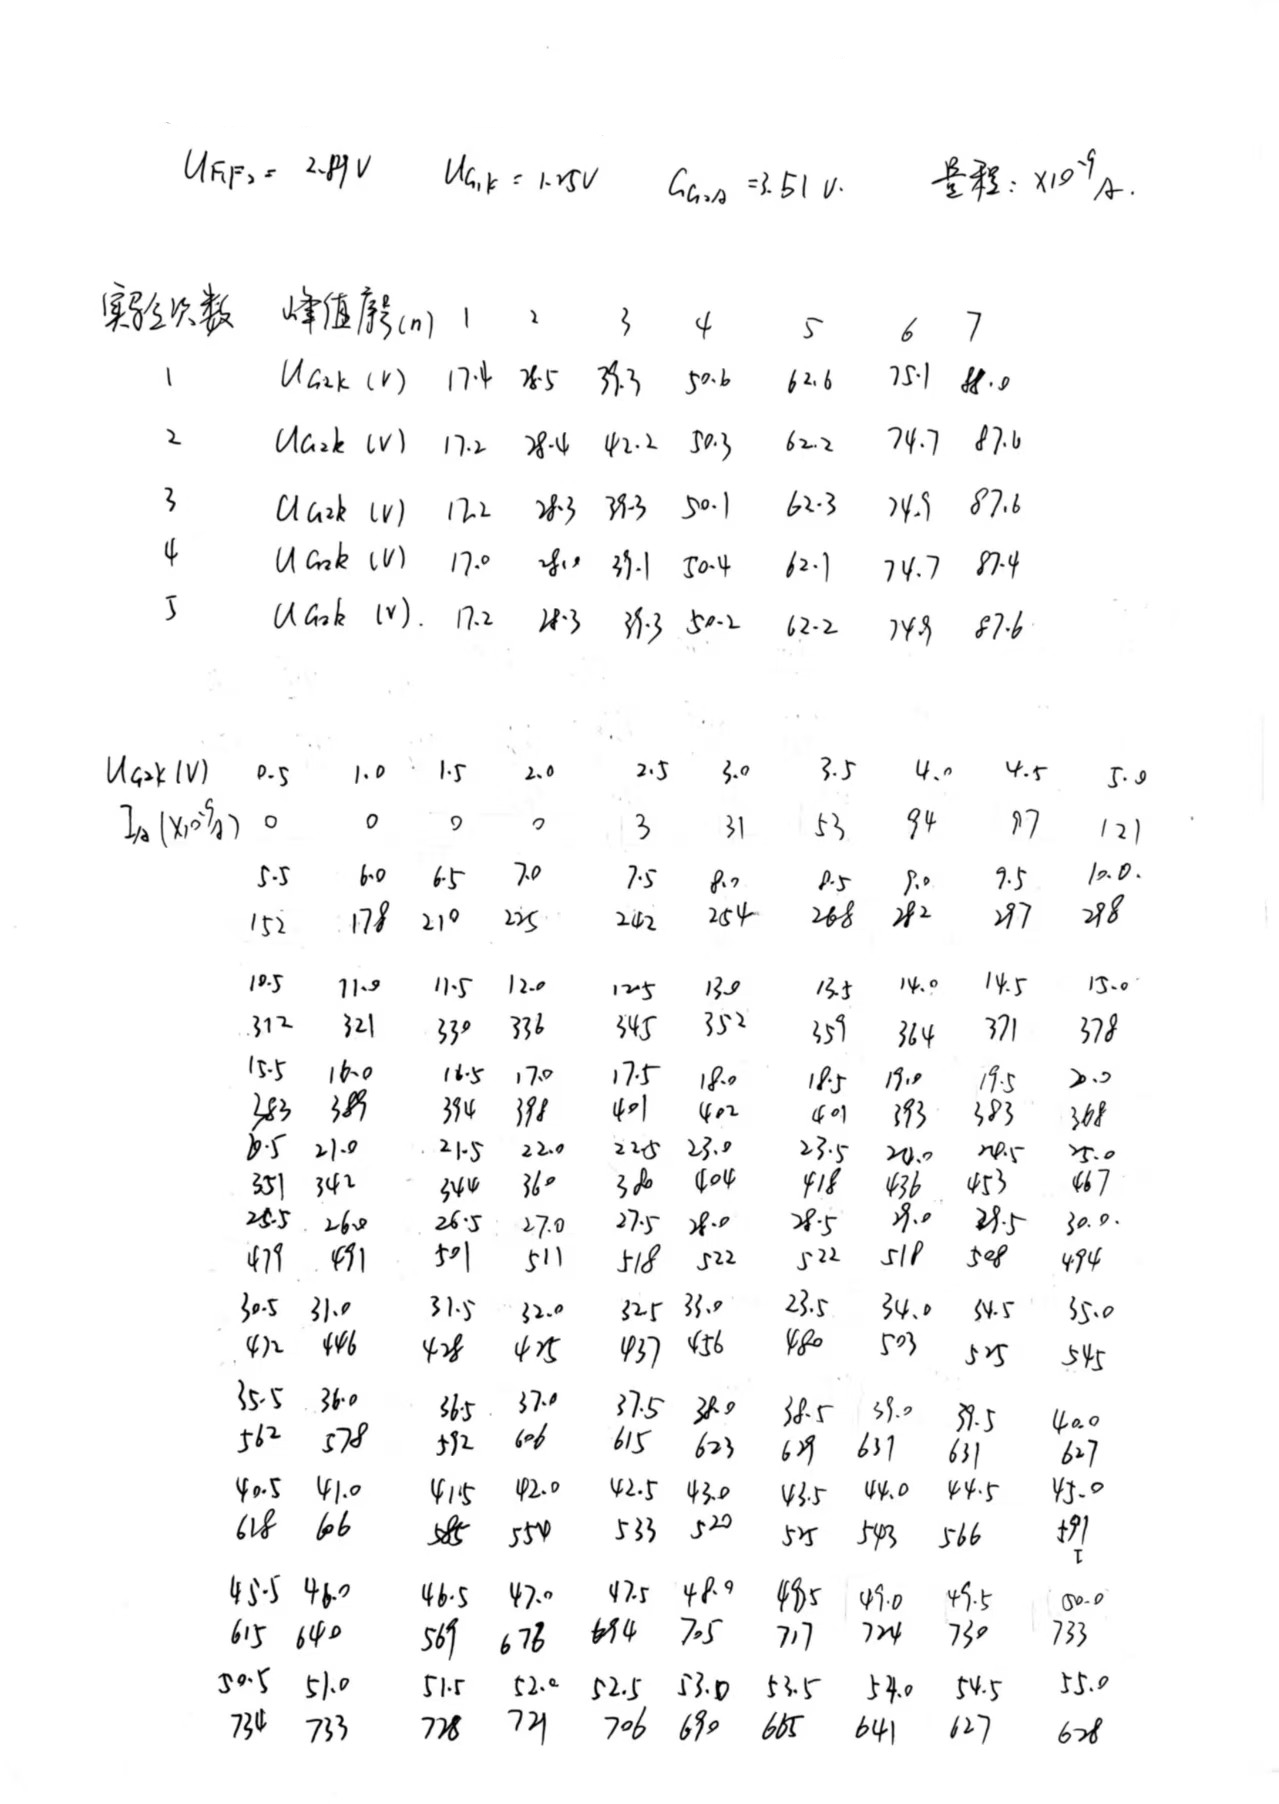
\includegraphics[width=13.5cm]{figures/实验数据1.jpg}
        \caption{实验数据}
        \label{fig:图2}
    \end{figure}

    \begin{figure}[htbp]
        \centering
        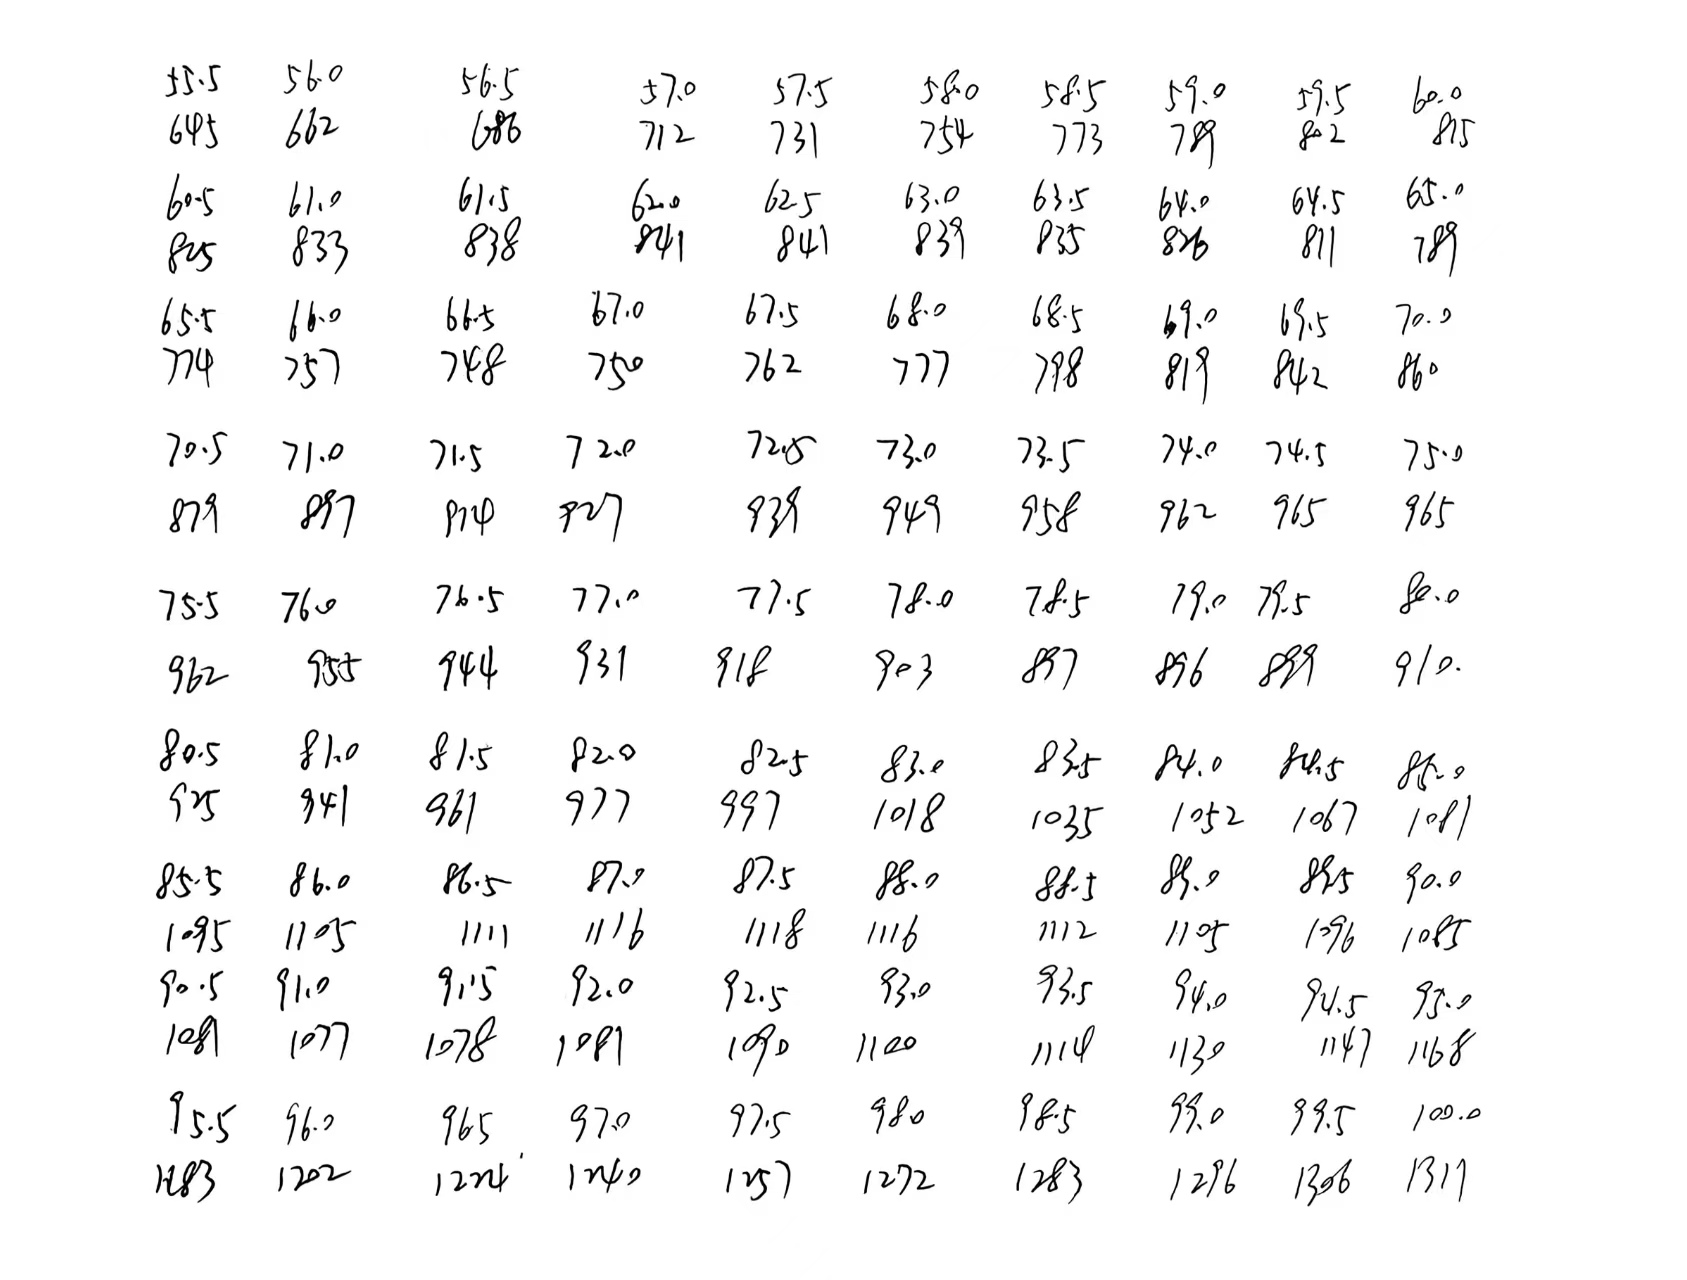
\includegraphics[width=13.5cm]{figures/实验数据2.jpg}
        \caption{实验数据}
        \label{fig:图2}
    \end{figure}

\newpage
    
\section{结果与分析}

    \subsection{数据处理与结果}
    \xiaosi （列出数据表格、选择数据处理方法、给定测量或计算结果，30分）
    
    \

     \subsubsection{自动测量数据处理}

    记录自动测量的峰值电压，得到如下表数据：

    \begin{table}[h!]
    \centering
    \caption{不同实验次数下的峰值电压 $U_{G2K}$ (V)}
    \vspace{0.2cm}
    \label{tab:peaks}
    \renewcommand{\arraystretch}{1.3}
    \begin{tabular}{c c c c c c c c}
        \toprule
        实验次数 & 峰值序号 $n=1$ & $n=2$ & $n=3$ & $n=4$ & $n=5$ & $n=6$ & $n=7$ \\
        \midrule
        1 & 17.4 & 28.5 & 39.3 & 50.6 & 62.6 & 75.1 & 88.0 \\
        2 & 17.2 & 28.4 & 42.2 & 50.3 & 62.2 & 74.7 & 87.6 \\
        3 & 17.2 & 28.3 & 39.3 & 50.1 & 62.3 & 74.9 & 87.6 \\
        4 & 17.0 & 28.1 & 39.1 & 50.4 & 62.1 & 74.7 & 87.4 \\
        5 & 17.2 & 28.3 & 39.3 & 50.2 & 62.2 & 74.9 & 87.6 \\
        \bottomrule
    \end{tabular}
\end{table}

对于每一组实验测得的 7 个峰值电压数据 $U_1, U_2, \dots, U_7$，利用逐差法计算第一激发电势 $U_0$。将数据分为前 3 个和后 3 个两组，对应峰值序号差为 $\Delta n = 4$。计算公式如下：
\begin{equation*}
    U_0 = \frac{(U_5 - U_1) + (U_6 - U_2) + (U_7 - U_3)}{3 \times 4} = \frac{\sum_{i=5}^{7} U_i - \sum_{j=1}^{3} U_j}{12}
\end{equation*}

根据表 1 数据，各次测量结果如下：

\begin{itemize}
    \item \textbf{第 1 次：} 
    $U_{0,1} = \frac{(62.6-17.4) + (75.1-28.5) + (88.0-39.3)}{12} \approx 11.708 \, \text{V}$
    
    \item \textbf{第 2 次：} 
    $U_{0,2} = \frac{(62.2-17.2) + (74.7-28.4) + (87.6-39.2)}{12} \approx 11.642 \, \text{V}$
    
    \item \textbf{第 3 次：} 
    $U_{0,3} = \frac{(62.3-17.2) + (74.9-28.3) + (87.6-39.3)}{12} \approx 11.667 \, \text{V}$
    
    \item \textbf{第 4 次：} 
    $U_{0,4} = \frac{(62.1-17.0) + (74.7-28.1) + (87.4-39.1)}{12} \approx 11.667 \, \text{V}$
    
    \item \textbf{第 5 次：} 
    $U_{0,5} = \frac{(62.2-17.2) + (74.9-28.3) + (87.6-39.3)}{12} \approx 11.658 \, \text{V}$
\end{itemize}

氩原子第一激发电势的平均值 $\overline{U_0}$ 为：
\begin{equation*}
    \overline{U_0} = \frac{1}{5} \sum_{k=1}^{5} U_{0,k} = \frac{11.708 + 11.642 + 11.667 + 11.667 + 11.658}{5} \approx \mathbf{11.67 \, \text{V}}
\end{equation*}

利用贝塞尔公式计算单次测量的实验标准偏差 $s$：
\begin{equation*}
    s = \sqrt{\frac{\sum_{k=1}^{n} (U_{0,k} - \overline{U_0})^2}{n-1}} \approx 0.0246 \, \text{V} \quad (n=5)
\end{equation*}

平均值的 A 类不确定度 $u_A$ 为：
\begin{equation*}
    u_A = \frac{s}{\sqrt{n}} = \frac{0.0246}{\sqrt{5}} \approx \mathbf{0.011 \, \text{V}}
\end{equation*}

本实验测得氩原子的第一激发电势为：
\begin{equation*}
    U_0 = \overline{U_0} \pm u_A = (11.67 \pm 0.01) \, \text{V}
\end{equation*}

\subsubsection{手动测量数据处理}

记录手动测量下$U_{G2K}$随$I_A$变化趋势，得到如下表数据：

\begin{table}[H]
    \centering
    \caption{手动扫描数据记录}
    \vspace{0.2cm}
    \label{tab:scan_data_6col}
    \renewcommand{\arraystretch}{1.0} % 稍微压缩行高
    % 使用 resizebox 自动缩放表格以适应页面宽度
    \resizebox{\textwidth}{!}{%
    \begin{tabular}{@{}cc | cc | cc | cc | cc | cc@{}}
        \toprule
        $U_{G2K}$ & $I_A$ & $U_{G2K}$ & $I_A$ & $U_{G2K}$ & $I_A$ & $U_{G2K}$ & $I_A$ & $U_{G2K}$ & $I_A$ & $U_{G2K}$ & $I_A$ \\
        \midrule
        0.5 & 0 & 17.5 & 401 & 34.5 & 525 & 51.5 & 728 & 68.5 & 798 & 85.5 & 1095 \\
        1.0 & 0 & 18.0 & 402 & 35.0 & 545 & 52.0 & 721 & 69.0 & 819 & 86.0 & 1105 \\
        1.5 & 0 & 18.5 & 401 & 35.5 & 562 & 52.5 & 706 & 69.5 & 842 & 86.5 & 1111 \\
        2.0 & 0 & 19.0 & 393 & 36.0 & 578 & 53.0 & 690 & 70.0 & 860 & 87.0 & 1116 \\
        2.5 & 3 & 19.5 & 383 & 36.5 & 592 & 53.5 & 665 & 70.5 & 879 & 87.5 & 1118 \\
        3.0 & 31 & 20.0 & 368 & 37.0 & 606 & 54.0 & 641 & 71.0 & 897 & 88.0 & 1116 \\
        3.5 & 53 & 20.5 & 351 & 37.5 & 615 & 54.5 & 627 & 71.5 & 914 & 88.5 & 1112 \\
        4.0 & 94 & 21.0 & 342 & 38.0 & 623 & 55.0 & 628 & 72.0 & 927 & 89.0 & 1105 \\
        4.5 & 97 & 21.5 & 346 & 38.5 & 629 & 55.5 & 645 & 72.5 & 939 & 89.5 & 1096 \\
        5.0 & 121 & 22.0 & 360 & 39.0 & 631 & 56.0 & 662 & 73.0 & 949 & 90.0 & 1085 \\
        5.5 & 152 & 22.5 & 380 & 39.5 & 631 & 56.5 & 686 & 73.5 & 958 & 90.5 & 1081 \\
        6.0 & 178 & 23.0 & 404 & 40.0 & 627 & 57.0 & 712 & 74.0 & 962 & 91.0 & 1077 \\
        6.5 & 210 & 23.5 & 418 & 40.5 & 618 & 57.5 & 731 & 74.5 & 965 & 91.5 & 1078 \\
        7.0 & 235 & 24.0 & 436 & 41.0 & 606 & 58.0 & 754 & 75.0 & 965 & 92.0 & 1081 \\
        7.5 & 242 & 24.5 & 453 & 41.5 & 585 & 58.5 & 773 & 75.5 & 962 & 92.5 & 1090 \\
        8.0 & 254 & 25.0 & 467 & 42.0 & 550 & 59.0 & 789 & 76.0 & 955 & 93.0 & 1100 \\
        8.5 & 268 & 25.5 & 479 & 42.5 & 533 & 59.5 & 802 & 76.5 & 944 & 93.5 & 1114 \\
        9.0 & 282 & 26.0 & 491 & 43.0 & 520 & 60.0 & 815 & 77.0 & 931 & 94.0 & 1130 \\
        9.5 & 297 & 26.5 & 501 & 43.5 & 525 & 60.5 & 825 & 77.5 & 918 & 94.5 & 1147 \\
        10.0 & 298 & 27.0 & 511 & 44.0 & 543 & 61.0 & 833 & 78.0 & 903 & 95.0 & 1168 \\
        10.5 & 312 & 27.5 & 518 & 44.5 & 566 & 61.5 & 838 & 78.5 & 887 & 95.5 & 1183 \\
        11.0 & 321 & 28.0 & 522 & 45.0 & 591 & 62.0 & 841 & 79.0 & 896 & 96.0 & 1202 \\
        11.5 & 330 & 28.5 & 522 & 45.5 & 615 & 62.5 & 841 & 79.5 & 899 & 96.5 & 1224 \\
        12.0 & 336 & 29.0 & 518 & 46.0 & 640 & 63.0 & 839 & 80.0 & 910 & 97.0 & 1240 \\
        12.5 & 345 & 29.5 & 508 & 46.5 & 669 & 63.5 & 835 & 80.5 & 925 & 97.5 & 1257 \\
        13.0 & 352 & 30.0 & 494 & 47.0 & 676 & 64.0 & 826 & 81.0 & 941 & 98.0 & 1272 \\
        13.5 & 359 & 30.5 & 472 & 47.5 & 694 & 64.5 & 811 & 81.5 & 961 & 98.5 & 1283 \\
        14.0 & 364 & 31.0 & 446 & 48.0 & 705 & 65.0 & 789 & 82.0 & 977 & 99.0 & 1296 \\
        14.5 & 371 & 31.5 & 428 & 48.5 & 717 & 65.5 & 774 & 82.5 & 997 & 99.5 & 1306 \\
        15.0 & 378 & 32.0 & 425 & 49.0 & 724 & 66.0 & 757 & 83.0 & 1018 & 100.0 & 1317 \\
        15.5 & 383 & 32.5 & 437 & 49.5 & 730 & 66.5 & 748 & 83.5 & 1035 & & \\
        16.0 & 389 & 33.0 & 456 & 50.0 & 733 & 67.0 & 750 & 84.0 & 1052 & & \\
        16.5 & 394 & 33.5 & 480 & 50.5 & 734 & 67.5 & 762 & 84.5 & 1067 & & \\
        17.0 & 398 & 34.0 & 503 & 51.0 & 733 & 68.0 & 777 & 85.0 & 1081 & & \\
        \bottomrule
    \end{tabular}%
    }
\end{table}

对上表数据进行拟合得到$U_{G2K}$随$I_A$变化的曲线，如下图：

\begin{figure}[H]
    \centering
    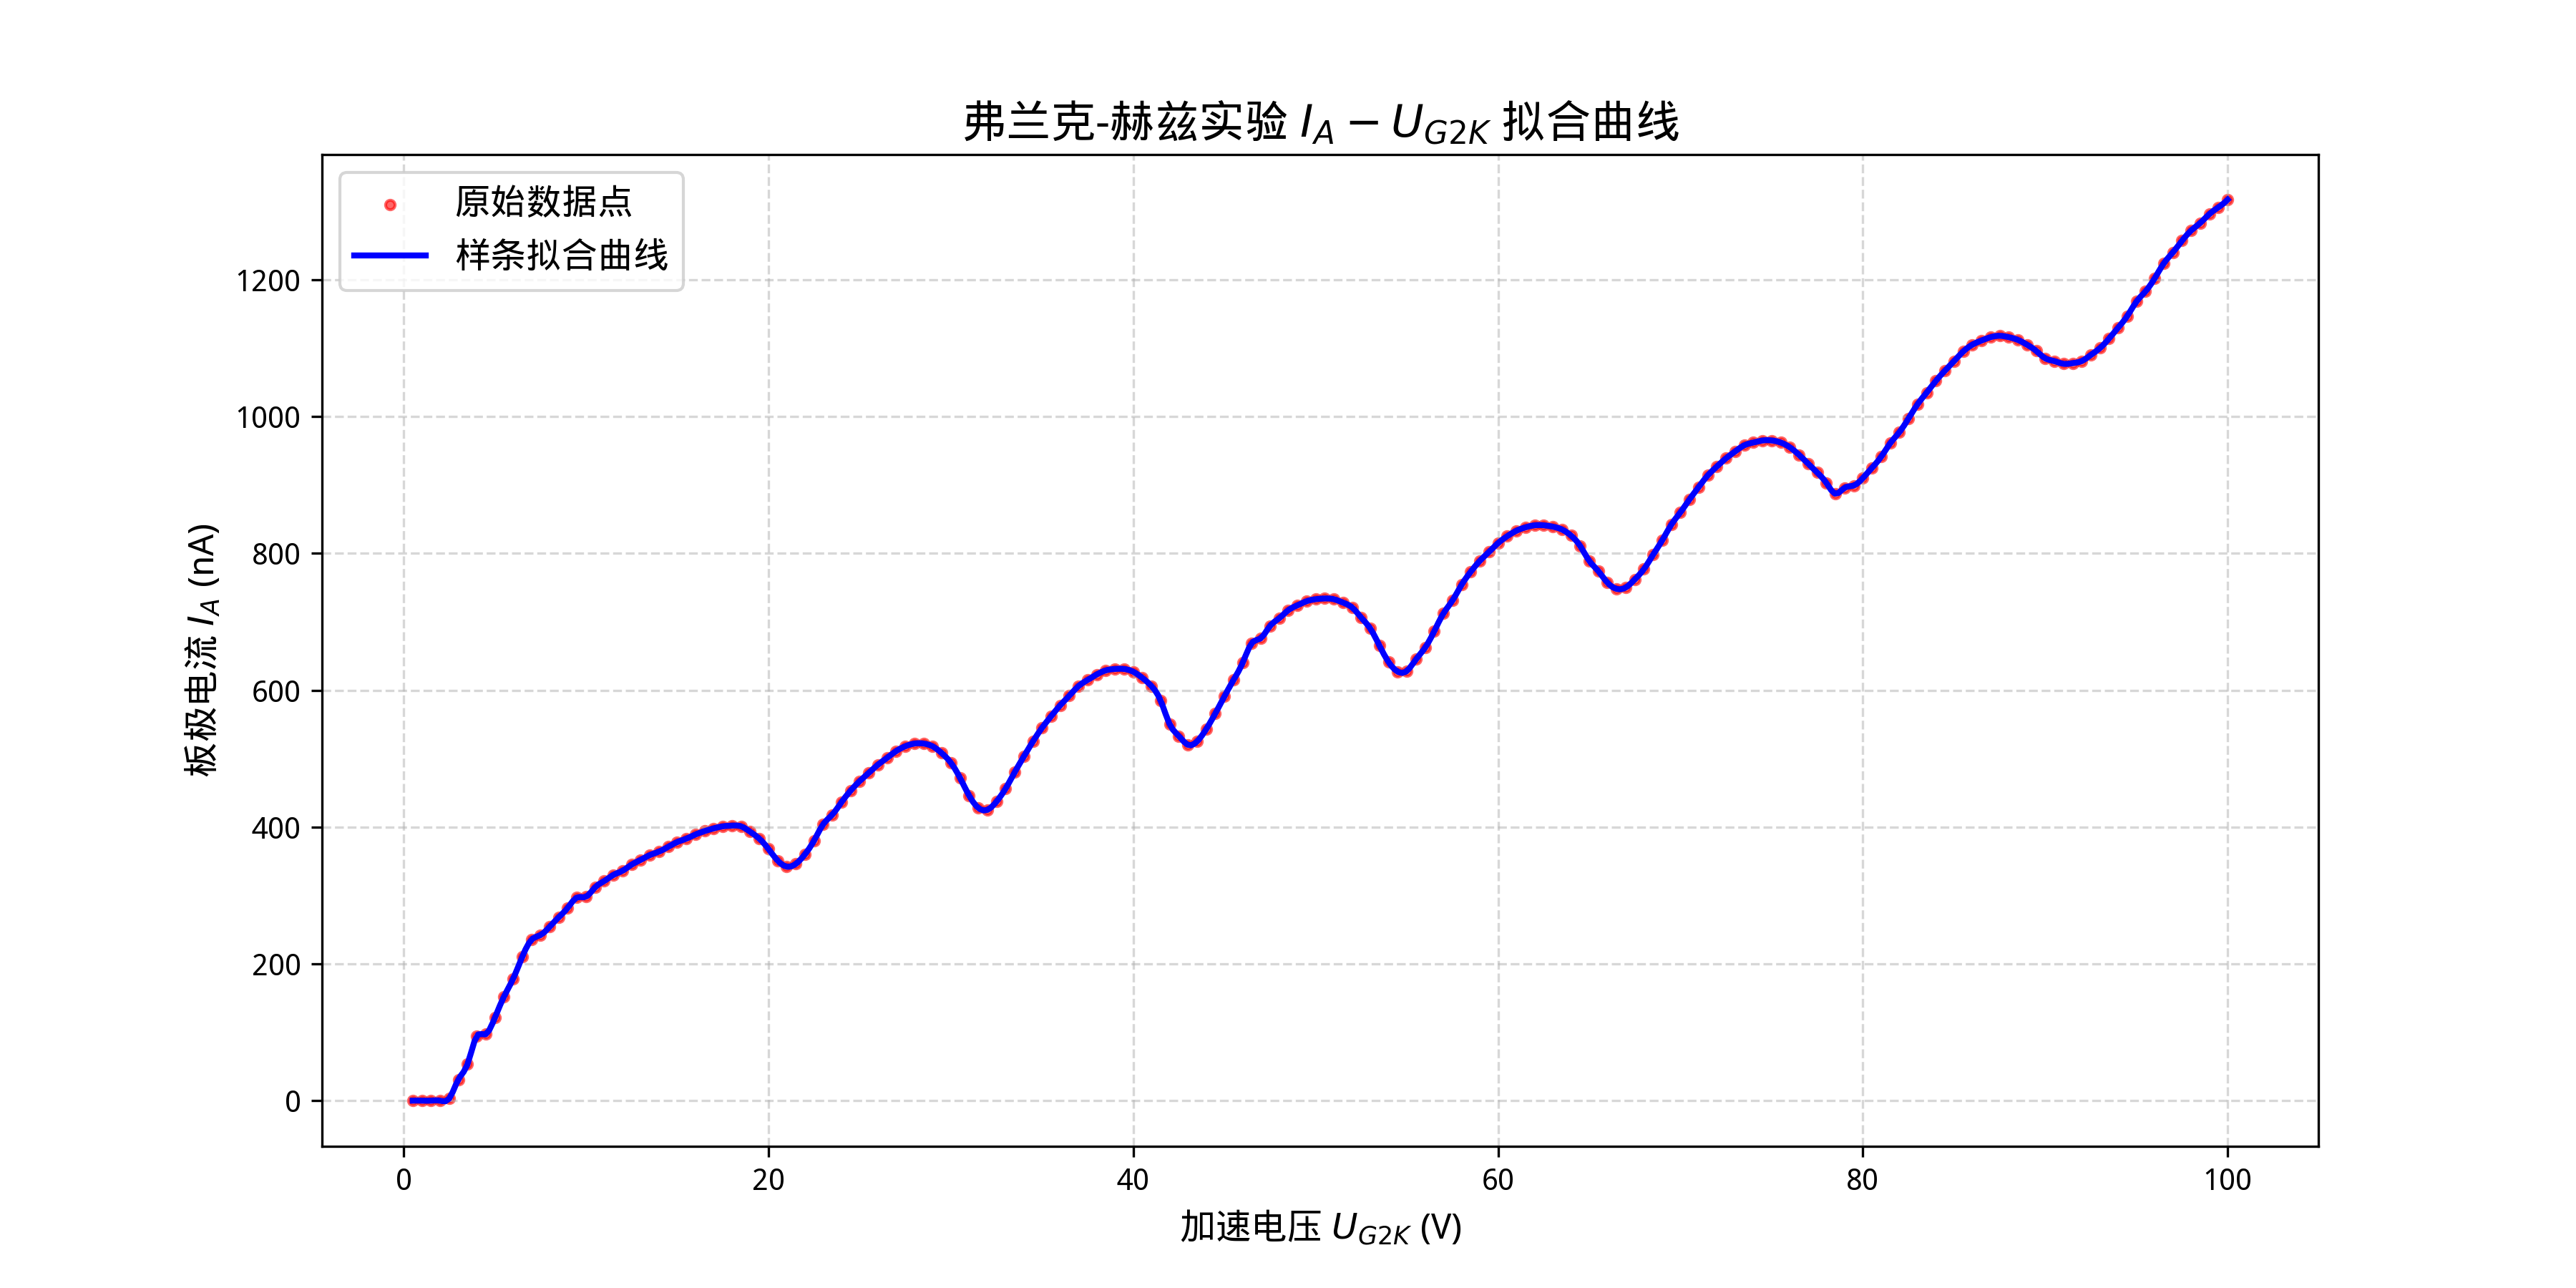
\includegraphics[width=18cm]{figures/franck_hertz_curve.png}
    \caption{$I_A$ - $U_{G2K}$曲线}
    \label{fig:principle2}
\end{figure}

根据$I_A$ - $U_{G2K}$曲线，找出各峰值电流对应的第二栅压$U_{G2K}$ 值，将峰值序号 $n$、第二栅压 $U_{G2K}$ 值记录在下表中：

\begin{table}[h]
    \centering
    \caption{各峰值点对应的第二栅压 $U_{G2K}$ 及电流 $I_A$}
    \vspace{0.2cm}
    \label{tab:peaks_scan}
    \renewcommand{\arraystretch}{1.3}
    \begin{tabular}{c c c}
        \toprule
        峰值序号 $n$ & $U_{G2K}$ (V) &  $I_A$ ($\times 10^{-9}$A) \\
        \midrule
        1 & 18.0 & 402 \\
        2 & 28.0 & 522 \\
        3 & 39.0 & 631 \\
        4 & 50.5 & 734 \\
        5 & 62.0 & 841 \\
        6 & 74.5 & 965 \\
        7 & 87.5 & 1118 \\
        \bottomrule
    \end{tabular}
\end{table}

选取前 6 个峰值数据 ($n=6$) 进行计算，分为两组：第一组为 $U_1, U_2, U_3$，第二组为 $U_4, U_5, U_6$。对应项相减的间隔为 $m=3$。

计算公式为：
\begin{equation}
    \overline{U_0} = \frac{(U_4 - U_1) + (U_5 - U_2) + (U_6 - U_3)}{3 \times m} = \frac{\sum_{i=1}^{3} (U_{i+3} - U_i)}{9}
\end{equation}

代入数据计算：
\begin{align*}
    U_4 - U_1 &= 50.5 - 18.0 = 32.5 \, \text{V} \\
    U_5 - U_2 &= 62.0 - 28.0 = 34.0 \, \text{V} \\
    U_6 - U_3 &= 74.5 - 39.0 = 35.5 \, \text{V} \\[1em]
    \overline{U_0} &= \frac{32.5 + 34.0 + 35.5}{9} \\
    &= \frac{102.0}{9} \\
    &\approx \mathbf{11.33 \, \text{V}}
\end{align*}

\textbf{所以，根据 $I_A - U_{G2K}$ 扫描曲线测得的氩原子第一激发电势为 11.33 V。}

    \subsection{误差分析}
    \xiaosi （运用测量误差、相对误差、不确定度等分析实验结果，20分）
    
    \begin{enumerate}
        \item 预热时间较短，导致测量值产生偏差；
        \item 设备老化，电容实际值与标称值的偏差，接触点的电阻等对实验结果产生影响；
        \item 灯管产生大量热量，导致电阻改变，影响实验结果。
    \end{enumerate}   
    
    \subsection{实验探讨}
    \xiaosi （对实验内容、现象和过程的小结，不超过100字，10分）

    \myspace{1}

    本次弗兰克-赫兹实验，我不仅掌握了测量仪器的使用方法，更通过手动扫描与自动测量，直观领略了电子与原子非弹性碰撞的物理图景。从绘制 $I_A-U_{G2K}$ 特性曲线、分析电流下降的物理机制，到处理峰值数据计算 $U_0$，每一个环节都要求极高的专注——比如在数据处理时理解并修正接触电势差带来的首峰偏移、保证读数准确性，这让我深刻体会到实验细节对结果可靠性的决定性影响，同时也锻炼了我对实验数据的分析与处理能力。
    
    \section{思考题}

    \xiaosi （解答教材或讲义或老师布置的思考题，10分）

    \subsubsection*{氩院子的第一激发态的物理意义是什么？}

    答：氩原子的第一激发电势在物理上代表了氩原子从基态跃迁到最低激发态所需的最小能量差（对应电压约为 11.5V 至 11.8V）。它标志着电子与氩原子发生非弹性碰撞并进行能量交换的阈值，即只有当外来电子的动能达到或超过这一数值时，氩原子才能吸收能量发生能级跃迁。这一特定的能量阈值直接证实了原子内部的能量状态是不连续的（即量子化的），为玻尔的原子能级理论提供了确凿的实验证据。

    \subsubsection*{温度对$I_A - U_{G2K}$曲线的影响如何？}

    答：温度主要决定了阴极发射热电子的数量以及电子的初动能分布。随着灯丝温度升高，阴极发射的电子数显著增多， 曲线的整体电流幅度会增大，便于观测；但若温度过高，会加剧阴极附近的空间电荷效应并导致电子能量分布变宽，使得曲线的峰谷变得平缓模糊（分辨率下降）甚至引起峰位偏移，从而影响测量精度。反之，温度过低则会导致板极电流微弱，信噪比差，难以观察到明显的周期性起伏。

\newpage

\sihao\textbf{注意事项：}
\xiaosi
\begin{enumerate}
    \item  用 PDF 格式上传“实验报告”，文件名：学生姓名+学号+实验名称+周次。
    \item  “实验报告”必须递交在“学在浙大”的本课程的对应实验项目的“作业”模块内。
    \item  “实验报告”成绩必须在“浙江大学物理实验教学中心网站”-“选课系统”内查询。
    \item 教学评价必须在“浙江大学物理实验教学中心网站”-“选课系统”内进行，学生必须进行教学评价，才能看到实验报告成绩，教学评价必须在本次实验结束后 3 天内进行。
\end{enumerate}

\vspace{1cm}
\xiaosi\centering \textbf{浙江大学物理实验教学中心制}

\end{document}